\documentclass[tikz,border=4pt]{standalone}
\usepackage{tikz}
\usetikzlibrary{arrows.meta}
\definecolor{nebula}{HTML}{6366F1}
\definecolor{spark}{HTML}{14B8A6}
\begin{document}
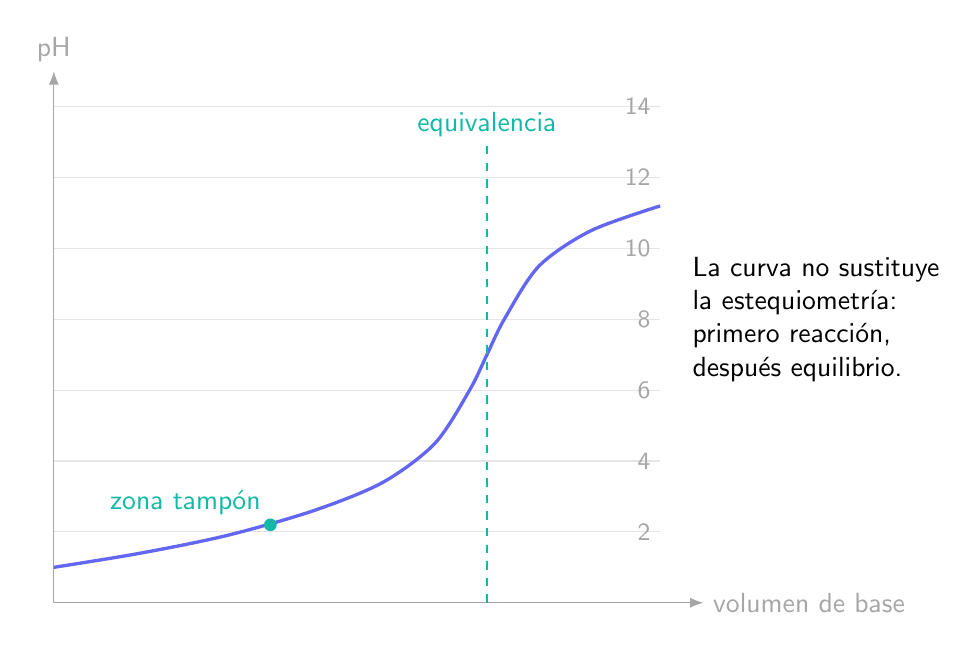
\begin{tikzpicture}[x=.11cm,y=.45cm,font=\sffamily,>=Latex]
  \draw[->,gray!70] (0,0)--(75,0) node[right] {volumen de base};
  \draw[->,gray!70] (0,0)--(0,15) node[above] {pH};
  \foreach \y in {2,4,6,8,10,12,14}\draw[gray!20](0,\y)--(70,\y) node[left,gray!70]{\small\y};
  \draw[very thick,nebula] plot[smooth] coordinates {(0,1)(10,1.4)(20,1.9)(30,2.6)(38,3.4)(44,4.5)(48,6)(50,7)(52,8)(56,9.5)(62,10.5)(70,11.2)};
  \draw[dashed,spark,thick] (50,0)--(50,13) node[above,fill=white,inner sep=1.5pt] {equivalencia};
  \fill[spark] (25,2.2) circle(2.3pt) node[above left] {zona tamp\'on};
  \node[align=left] at (88,8) {La curva no sustituye\\la estequiometr\'ia:\\primero reacci\'on,\\despu\'es equilibrio.};
\end{tikzpicture}
\end{document}
